\documentclass[aspectratio=169]{beamer}

% ---------- Beamer theme ----------
\usetheme{metropolis} % If you don't have it, switch to: \usetheme{default}
\metroset{block=fill,progressbar=frametitle}

% ---------- Encoding & typography ----------
\usepackage[T1]{fontenc}
\usepackage[utf8]{inputenc}
\usepackage{microtype}

% ---------- Graphics / Tables ----------
\usepackage{graphicx}
\usepackage{booktabs}
\usepackage{array}
\usepackage{xcolor}

% ---------- Code listings ----------
\usepackage{listings}
\lstdefinestyle{tinyterminal}{
  basicstyle=\ttfamily\small,
  columns=fullflexible,
  keepspaces=true,
  showstringspaces=false,
  frame=single,
  breaklines=true,
  framerule=.2pt,
  rulecolor=\color{black!30},
  keywordstyle=\bfseries\color{blue!60!black},
  commentstyle=\itshape\color{green!40!black},
  stringstyle=\color{red!60!black}
}
\lstdefinelanguage{Arduino}{
  morekeywords={pinMode,digitalWrite,analogRead,delay,millis,Serial,WiFi,WiFiS3,WiFiSSLClient,HttpClient,MqttClient},
  sensitive=true,
  morecomment=[l]{//},
  morecomment=[s]{/*}{*/},
  morestring=[b]"
}
\lstdefinelanguage{JSON}{
  morestring=[b]",
  morecomment=[l]{//},
  literate=
   {*}{*}1
   {:}{:}1
   {,}{,}1
   {\{}{{\{}}1
   {\}}{{\}}}1
}

% ---------- Title ----------
\title{APIs Overview for Arduino}
\subtitle{UNO R4 WiFi • REST • MQTT • Security • Best Practices}
\author{Anatolie Jentimir — BHCC STEM Club}
\date{\today}

\begin{document}
\maketitle

% =========================================================
\begin{frame}{Why APIs for Arduino?}
APIs (Application Programming Interfaces) are the bridge between your Arduino and:
\begin{itemize}
  \item Cloud services \& databases (data logging, analytics, dashboards)
  \item Mobile / web apps (real-time monitoring \& control)
  \item Other devices (gateway nodes, microservices)
\end{itemize}
\medskip
\textbf{Smart Garden example}: DHT11 + soil sensor $\rightarrow$ publish via API $\rightarrow$ store \& visualize $\rightarrow$ alerts \& ML predictions.
\end{frame}

% =========================================================
\begin{frame}{API Communication Models}
\begin{tabular}{>{\bfseries}m{2.8cm} m{2.3cm} m{2.5cm} m{6.7cm}}
Type & Protocol & Direction & When to use \\
\midrule
REST API & HTTP/HTTPS & Client$\rightarrow$Server & Simple JSON posts, easy web backends (FastAPI/Flask/Supabase). \\
MQTT API & TCP/TLS & Pub/Sub (bi-dir) & Low-power IoT telemetry, scalable, commands via topics. \\
WebSocket & TCP & Bi-directional & Realtime dashboards pushing updates to browsers. \\
GraphQL & HTTP/HTTPS & Client$\rightarrow$Server & Query only the fields you need; less common on MCUs. \\
\end{tabular}
\end{frame}

% =========================================================
\section{REST APIs}
\begin{frame}{REST: Concept}
\textbf{Endpoints:} \texttt{/ingest}, \texttt{/telemetry}, \texttt{/status}\quad
\textbf{Methods:} \texttt{GET, POST, PUT, DELETE}
\medskip

\begin{block}{Typical flow}
\begin{enumerate}
  \item Arduino formats sensor data as JSON.
  \item Sends HTTPS \texttt{POST} to server endpoint.
  \item Server authenticates (API key), validates schema, stores data.
  \item Optional: server responds with status or commands.
\end{enumerate}
\end{block}
\end{frame}

\begin{frame}[fragile]{UNO R4 WiFi: Minimal HTTPS POST (REST)}
\textbf{Libraries}: \texttt{WiFiS3}, \texttt{ArduinoHttpClient}
\begin{lstlisting}[language=Arduino,style=tinyterminal]
#include <WiFiS3.h>
#include <ArduinoHttpClient.h>

const char* SSID = "YOUR_SSID";
const char* PASS = "YOUR_PASS";

const char* HOST = "api.example.com";
const int   PORT = 443; // HTTPS
const char* API_KEY = "YOUR_LONG_RANDOM_KEY";

WiFiSSLClient net;         // TLS
HttpClient    client(net, HOST, PORT);

void setup() {
  Serial.begin(115200);
  WiFi.begin(SSID, PASS);
  while (WiFi.status() != WL_CONNECTED) delay(250);
}

void loop() {
  String body = "{\"nodeId\":\"SOIL1\",\"temperature\":23.8,"
                "\"humidity\":41.2,\"soilMoisture\":0.31}";

  client.beginRequest();
  client.post("/ingest");
  client.sendHeader("Content-Type", "application/json");
  client.sendHeader("Authorization", String("Bearer ") + API_KEY);
  client.sendHeader("Content-Length", body.length());
  client.beginBody();
  client.print(body);
  int ok = client.endRequest();

  int code = client.responseStatusCode();
  Serial.println(code);
  client.stop();
  delay(5000);
}
\end{lstlisting}
\end{frame}

\begin{frame}[fragile]{FastAPI: Simple Ingest Endpoint (Server)}
\begin{lstlisting}[language=Python,style=tinyterminal]
from fastapi import FastAPI, Request, HTTPException

app = FastAPI()
EXPECTED = "YOUR_LONG_RANDOM_KEY"

@app.post("/ingest")
async def ingest(req: Request):
    auth = req.headers.get("authorization", "")
    if not auth.startswith("Bearer ") or auth.split(" ", 1)[1] != EXPECTED:
        raise HTTPException(status_code=401, detail="invalid api key")

    data = await req.json()
    # TODO: validate schema & ranges, then write to DB
    return {"ok": True, "size": len(str(data))}
\end{lstlisting}
\end{frame}

% =========================================================
\section{MQTT APIs}
\begin{frame}[fragile]{MQTT: Concept}
\begin{columns}[T,onlytextwidth]
\column{0.55\textwidth}
\textbf{Broker-centric pub/sub}
\begin{itemize}
  \item Devices \textit{publish} telemetry to topics.
  \item Dashboards/servers \textit{subscribe} to topics.
  \item Lightweight, low bandwidth, great for fleets.
\end{itemize}
\medskip
\textbf{Topic design}
\begin{lstlisting}[language={},style=tinyterminal]
bhcc/smartgarden/SOIL1/telemetry
bhcc/smartgarden/SOIL1/status
bhcc/smartgarden/SOIL1/command
\end{lstlisting}

\column{0.45\textwidth}
\textbf{Flow}
\begin{lstlisting}[language={},style=tinyterminal]
[UNO R4] --publish--> [MQTT Broker]
      \                   /
       \--subscribe<-----/
           [Server/Dash]
\end{lstlisting}
\end{columns}
\end{frame}

\begin{frame}[fragile]{UNO R4 WiFi: MQTT over TLS}
\textbf{Libraries}: \texttt{WiFiS3}, \texttt{ArduinoMqttClient}
\begin{lstlisting}[language=Arduino,style=tinyterminal]
#include <WiFiS3.h>
#include <ArduinoMqttClient.h>

const char* SSID = "YOUR_SSID";
const char* PASS = "YOUR_PASS";
const char* BROKER = "broker.example.com";
const int   PORT   = 8883;  // TLS
const char* USER   = "SOIL1";
const char* TOKEN  = "YOUR_LONG_RANDOM_KEY";

WiFiSSLClient net;
MqttClient    mqtt(net);

void setup() {
  WiFi.begin(SSID, PASS);
  while (WiFi.status() != WL_CONNECTED) delay(200);

  mqtt.setId("uno-r4-soil1");
  mqtt.setUsernamePassword(USER, TOKEN); // API key as password
  while (!mqtt.connect(BROKER, PORT)) delay(500);
}

void loop() {
  mqtt.poll();
  mqtt.beginMessage("bhcc/smartgarden/SOIL1/telemetry", false, 1);
  mqtt.print("{\"t\":23.8,\"h\":41.2,\"s\":0.31}");
  mqtt.endMessage();
  delay(5000);
}
\end{lstlisting}
\end{frame}

% =========================================================
\section{WebSockets (optional)}
\begin{frame}{WebSockets: When to Use}
\begin{itemize}
  \item Real-time dashboards pushing updates to browsers.
  \item For Arduino, typically proxied via a gateway (ESP32/PC server).
  \item Security and framing overhead can be higher than MQTT.
\end{itemize}
\end{frame}

% =========================================================
\section{Authentication \& Security}
\begin{frame}{API Keys \& Practical Security}
\textbf{API key placement}
\begin{itemize}
  \item HTTP header: \texttt{Authorization: Bearer \textit{KEY}} (recommended)
  \item Query string: \texttt{?api\_key=KEY} (only if service requires)
  \item MQTT username/password: \texttt{user=deviceId}, \texttt{pass=KEY}
\end{itemize}
\medskip
\textbf{Checklist}
\begin{enumerate}
  \item Use \textbf{TLS} (HTTPS / MQTT over TLS).
  \item One \textbf{unique key per device}; rotate keys.
  \item Server-side \textbf{validation}: schema, ranges, rate limit.
  \item Include \textbf{timestamps}; reject stale data.
  \item Avoid printing secrets on Serial in production.
\end{enumerate}
\end{frame}

% =========================================================
\section{Best Practices}
\begin{frame}{Robustness \& Data Quality}
\begin{itemize}
  \item \textbf{Retry buffers}: cache unsent readings when offline.
  \item \textbf{QoS 1} for MQTT telemetry; use retained only for last-known status.
  \item \textbf{Batch uploads}: send N readings per POST to reduce overhead.
  \item \textbf{Retention policies}: downsample older data in TSDB (e.g., InfluxDB).
  \item \textbf{Observability}: add device status pings and error counters.
\end{itemize}
\end{frame}









% % =========================================================
% \section{Architecture}
% \begin{frame}{End-to-End Reference Architecture}
% \begin{lstlisting}[language={},style=tinyterminal]
% ┌────────────────────────────┐
% │  Arduino UNO R4 WiFi       │  Sensors: DHT11, Soil, etc.
% │  ├─ WiFiS3 (HTTPS/MQTT)    │
% └──────────────┬─────────────┘
%                │
%          HTTPS / MQTT (TLS)
%                │
% ┌────────────────────────────┐     ┌───────────────────────────┐
% │     API / Broker Layer     │     │  Processing / Storage     │
% │  ├─ FastAPI / Nginx (REST) │◄──► │  InfluxDB / PostgreSQL    │
% │  └─ EMQX / Mosquitto (MQTT)│     │  Telegraf / Workers       │
% └──────────────┬─────────────┘     └──────────────┬────────────┘
%                │                                   │
%                ▼                                   ▼
%         ┌───────────────┐                   ┌──────────────┐
%         │  Grafana      │  Dashboards       │  RStudio/ML  │  Analytics/AI
%         └───────────────┘                   └──────────────┘
% \end{lstlisting}
% \end{frame}







% =========================================================
\section{Architecture}
\begin{frame}{End-to-End Reference Architecture}
\centering
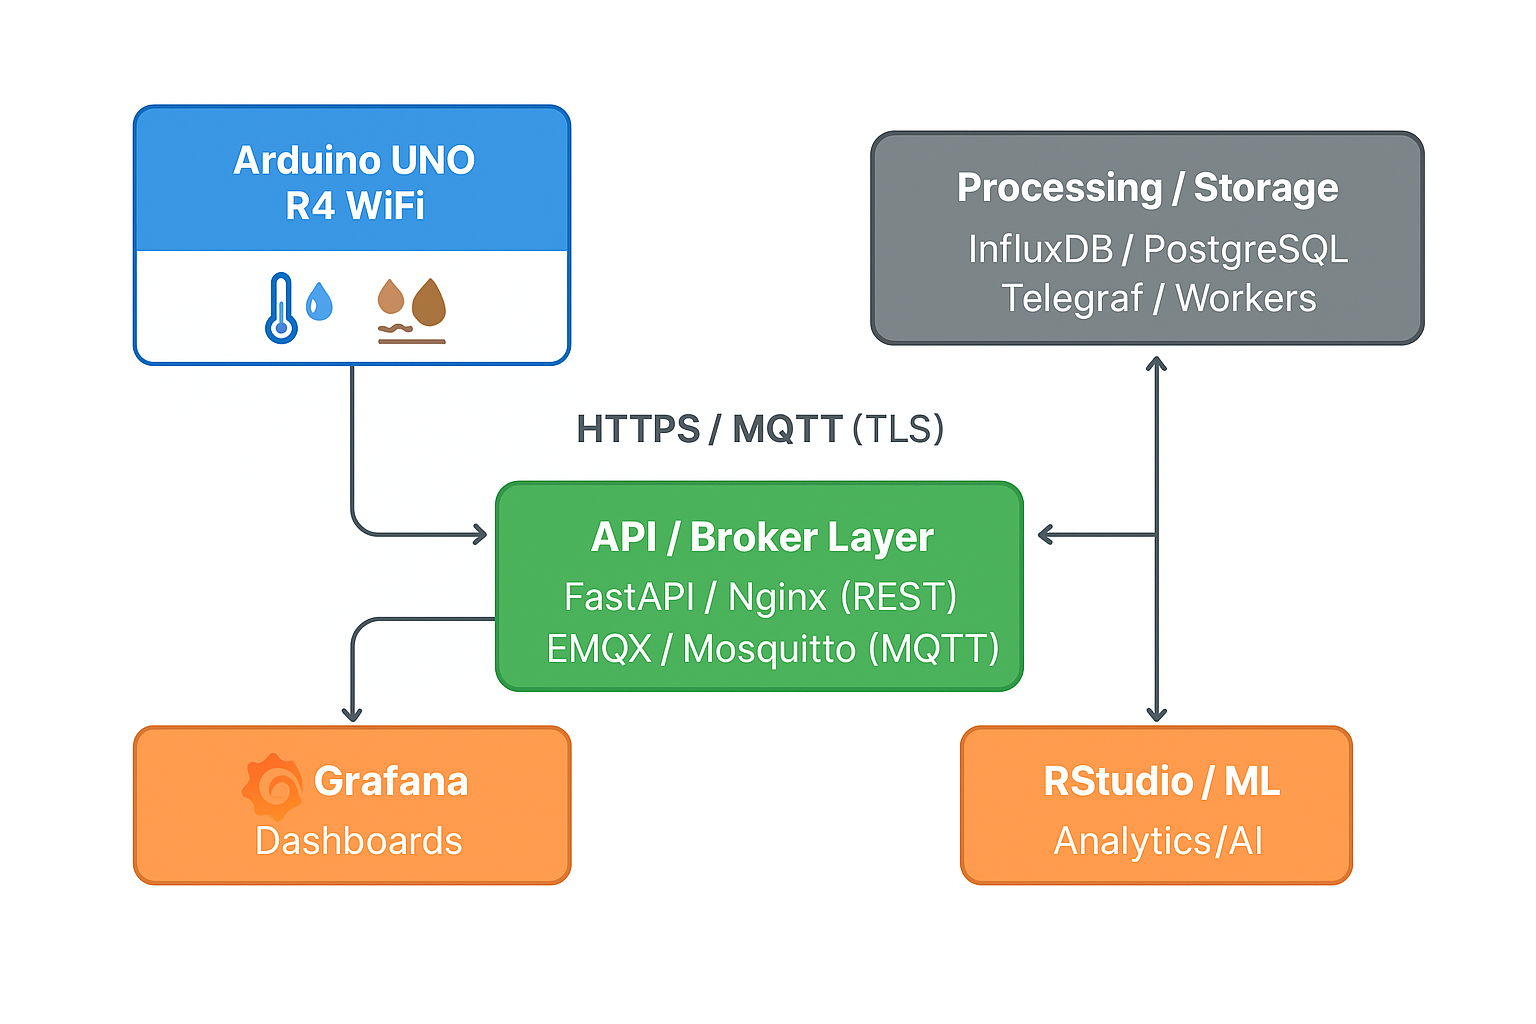
\includegraphics[width=\linewidth]{A_flowchart_diagram_in_a_digital_vector_illustrati.png}
\end{frame}







% =========================================================
\section{Practical Examples}
\begin{frame}{Service Examples \& Endpoints}
\begin{tabular}{>{\bfseries}m{3.0cm} m{3.5cm} m{7.5cm}}
Platform & Method & Example \\
\midrule
ThingSpeak & REST & \texttt{/update?api\_key=XXX\&field1=23.5} \\
Arduino IoT Cloud & MQTT & \texttt{deviceId/variableName} (provisioned) \\
Supabase (Postgres) & REST & \texttt{/rest/v1/sensors} (insert JSON rows) \\
Custom (FastAPI) & REST & \texttt{/ingest}, \texttt{/telemetry} \\
\end{tabular}
\end{frame}

\begin{frame}[fragile]{JSON Payload Template}
\begin{lstlisting}[language=JSON,style=tinyterminal]
{
  "ts": 1730132405,
  "nodeId": "SOIL1",
  "temperature": 23.8,
  "humidity": 41.2,
  "soilMoisture": 0.31,
  "vbat": 4.86,
  "rssi": -62
}
\end{lstlisting}
\textit{Tip:} Keep field names short but clear; include a UNIX timestamp and a device identifier.
\end{frame}

% =========================================================
\section{Troubleshooting}
\begin{frame}{Common Issues \& Fixes}
\begin{tabular}{>{\bfseries}m{4.2cm} m{8.6cm}}
Symptom & Fix \\
\midrule
\texttt{connection failed} / timeouts & Verify SSID/password, DNS/host, open outbound ports (443/8883). \\
\texttt{401/403 Unauthorized} & Check API key location (header vs query), token validity/rotation. \\
Duplicate MQTT data & Ensure retained flag is off for telemetry; use QoS1 only if needed. \\
Malformed JSON & Validate braces/quotes; avoid trailing commas; check decimal dots. \\
Clock skew / stale data & Sync NTP or include controller timestamp; reject stale on server. \\
\end{tabular}
\end{frame}

% =========================================================
\section{Advanced Extensions}
\begin{frame}{Beyond the Basics}
\begin{itemize}
  \item \textbf{OTA updates}: Arduino IoT Cloud or custom HTTPS fetcher.
  \item \textbf{JWT / HMAC}: signed requests (anti-replay, integrity).
  \item \textbf{Edge batching \& compression}: send fewer, larger posts.
  \item \textbf{Alerts}: Grafana/Influx tasks or server rules (email/Telegram).
  \item \textbf{AI loop}: export to CSV $\rightarrow$ RStudio/ML $\rightarrow$ predictions via API.
\end{itemize}
\end{frame}

% =========================================================
\section{Summary}
\begin{frame}{Key Takeaways}
\begin{itemize}
  \item REST = simplest path to any web backend; MQTT = best for IoT scale.
  \item Use TLS, per-device API keys, and server-side validation.
  \item Design clean topics/endpoints and stable JSON schemas.
  \item Plan dashboards, retention, and ML integration from day one.
\end{itemize}
\end{frame}

\begin{frame}{References}
\begin{itemize}
  \item Arduino Docs — \texttt{https://docs.arduino.cc}
  \item MQTT — \texttt{https://mqtt.org}
  \item ThingSpeak — \texttt{https://thingspeak.com/docs}
  \item InfluxData — \texttt{https://www.influxdata.com}
  \item FastAPI — \texttt{https://fastapi.tiangolo.com}
\end{itemize}
\end{frame}

\begin{frame}[standout]
Questions? \newline
\small Anatolie Jentimir — BHCC STEM Club
\end{frame}

\end{document}
